\chapter{Conclusion and Recommendation}
\section{Conclusion}
Cybersecurity is a complex field and threat actors are ever evolving their tradecraft in clever ways. Every single
running business is not too small to be attacked, but they may be too small for them to make the news. Therefore, transparency
to the clients is important, because lack of visibility to the clients can lead to a loss of trust. This graduation project serves
as the first iteration by \acrshort{qict} about the integration of SentinelOne to its internal application, the \acrshort{qaas} app.

The \acrshort{qaas} app is a cloud-based application that is used by \acrshort{qict} to provide a better service to their clients.
The app itself is a multi-tenant application, meaning that it can be used by multiple clients at the same time. The app is made
using Flutter, a cross-platform framework that is developed by Google, and Firebase as the back-end cloud solution. The app itself
has several modules that are used by different user roles, such as the clients, the helpdesk, and the \acrshort{it} admins. The app
is also integrated with several \acrshort{api}s, such as the N-Central, Resello, Snelstart, Bodyguard.io, and PerfectView. The app
also uses Algolia, an \acrshort{ai} powered search engine, to make the search faster and more accurate by allowing typos.

The \acrshort{qaas} app itself has 3 different user roles in its system: the clients, the helpdesk, and the \acrshort{it} admins.
Alongside that, there are also modules, user tags, and templates. Modules are basically the page view of the app, assigning modules
to an appropriate user role is done by the \acrshort{it} admins. User tags are assigned to a user to give them permission to see
or edit certain modules. Templates

SentinelOne is a cybersecurity company based in California, United States that has a product of the same name. It is an \acrshort{edr}
platform, which purpose is to detect and respond to threats of an endpoint in real-time, replacing the traditional \acrshort{av}.
It utilizes \acrshort{ai} and \acrshort{ml} on an Agent to detect and respond to threats, and it is deployed on the endpoint itself.
The purpose of an \acrshort{edr} platform is to have a centralized view of all the endpoints that are connected to the platform, and
to provide real-time monitoring of the threats that are detected by the Agent. The platform itself is also integrated with several
\acrshort{api}s, such as the \acrshort{api} for the Agents for endpoints, the Rangers for networks, and the application management,
each data is uniquely processed and stored in separate \acrshort{db}s.

SentinelOne \acrshort{edr} platform is possible to be integrated with the \acrshort{qaas} app, which was made in Flutter with
Firebase as the back-end cloud solution, utilizing SentinelOne \acrshort{api} to fetch the data. In order that this \acrshort{api}
to be able to send the correct data, the necessary Agents and Ranger need to be set up properly in a client's machine. This Agent will
then gather the data from the client's machine and send it to the management \acrshort{db}, providing real-time monitoring. Additionally,
a SentinelOne account with the necessary rights to read the data with its \acrshort{api} key is also needed to be configured. Lastly, a
SentinelOne \acrshort{api} key that is based on a SentinelOne account needs to be set up with a proper role to read the data, and secured
in  the cloud where it is encrypted like Google Secret Manager or Azure Key Vault.

Based on comparison with other \acrshort{edr} platforms, it is concluded that when making a visual representation for the users, it is
important that the images are understandable and user-friendly to the users to create a strong message when displaying a complex data
or information. The visualization widget also needs to be customizable, so that the user can choose which data they want to see in the
dashboard. The colours of these visualization widgets do not need to be too flashy, as it can distract the user from the data itself. Instead,
opting for colour that is more suitable to the general theme of the app is preferable. In the front-end, the visualization is done using the
Flutter framework. The framework itself have several packages that can do this: \textit{fl\_chart}, \textit{syncfusion\_flutter\_charts},
and \textit{flutter\_echarts}. The author chose to use all the three packages as all of them have their own strengths and weaknesses, along
with making customization options for the user to choose which types of visualization and what data they want to see.

In the back-end, several functions with different functionalities need to be created to handle the data that is fetched from different
SentinelOne \acrshort{api} endpoints. The user's session and preference data are stored in the Firebase Firestore \acrshort{db}, and as
well as \acrshort{ai} powered Algolia search engine to make the search faster and more accurate. Additional features such as filtering,
sorting, and pagination will be handled by inputting the correct headers to the \acrshort{api} request.

\section{Recommendation}

\subsection{Integration with N-Central data}

In the research phase of this project, the Company Supervisor mentioned that there are some issues regarding the data coming
from N-Central \acrshort{api} (which also one of the \acrshort{api} used for security) that sometimes can cause data discrepancy. The author
has looked into some N-Central data and noticed some similarities with some SentinelOne data structure. The idea of this recommendation
is to combine the data from SentinelOne and N-Central that have similar structure, to then make the data to be more accurate and reliable.

For example, N-Central has one \acrshort{api} that can automatically check for an update of an application
of a device, given the correct application \acrshort{id} and device \acrshort{id}. If a device has an outdated application, it can either
update the application automatically, or notify the corresponding user. If the device also has a SentinelOne Agent installed, the Agent
can then detect all the applications that are installed and know immediately if there is an outdated application, with checking for the
outdated application that may pose a security risk according to the fastest \acrshort{cve} database. Combining two of these functionalities
would then make sense, as SentinelOne can then prioritize outdated applications on a device, and N-Central can then notify the user
to update the said application. This way, the user can then have a more secure device, and the \acrshort{qaas} app can then provide a more
comprehensive security solution to the user.

\subsection{Redis middleware NoSQL database caching}

Redis is a powerful tool for \acrshort{db} that uses in-memory data structure to provide caching and message broker. It supports
various data structures (\textit{\cite{redisDataStructure}}), such as strings, hashes, lists, sorted sets, with range queries,
bitmaps, hyperlogs, geospatial indexes with radius queries, and streams.

Because the main idea in Redis is to provide caching of the data, coupled with the fact that it is a \acrshort{nosql} \acrshort{db},
Redis is exceptionally fast to query due to its in-memory nature in contrast to traditional disk-based \acrshort{db}s. This makes it
suitable for use cases where low latency and high throughput are required, making it perfect for getting and storing data that is
frequently accessed.

The idea is to put SentinelOne data into the Redis \acrshort{db} too, with the limit of 5-10 minutes before the cache is deleted,
and then fetch the data from the Redis \acrshort{db} instead of directly fetching it from Firestore and SentinelOne \acrshort{api}
constantly. Implementing Redis will make querying the data faster than Firestore, providing better \acrshort{ux} for the users.

However, there is one potential downside that the author sees when using Redis in this project. According to these articles
(\textit{\cite{redisIsNoLongerFree}}, and \textit{\cite{redisMomento}}), as of March 2024, Redis is no  longer open source. They
changed the official licence for all future versions. This has serious consequences for the open-source community and some companies
providing managed Redis. Therefore, the initial development of the Redis middleware to this project can no longer use the free version
of Redis from a Redis provider without a direct partnership with Redis. Nonetheless, with a direct paid subscription to Redis, the
author believes that in the long run, using Redis as a means of caching the data will be beneficial for the \acrshort{qaas} app,
especially when the number of customers have grown and the SentinelOne data gets called more frequently.



\begin{figure}[htbp]
  \centering
  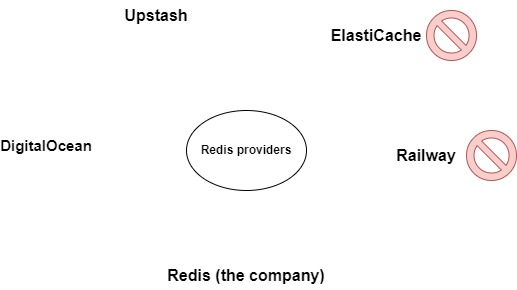
\includegraphics[width=0.9\textwidth]{Figures/Redis Providers.jpg}
  \caption{Redis providers now cannot distribute Redis anymore without a direct partnership with Redis, thefore Redis itself controlling
    the pricing.}
\end{figure}


\begin{figure}[htbp]
  \centering
  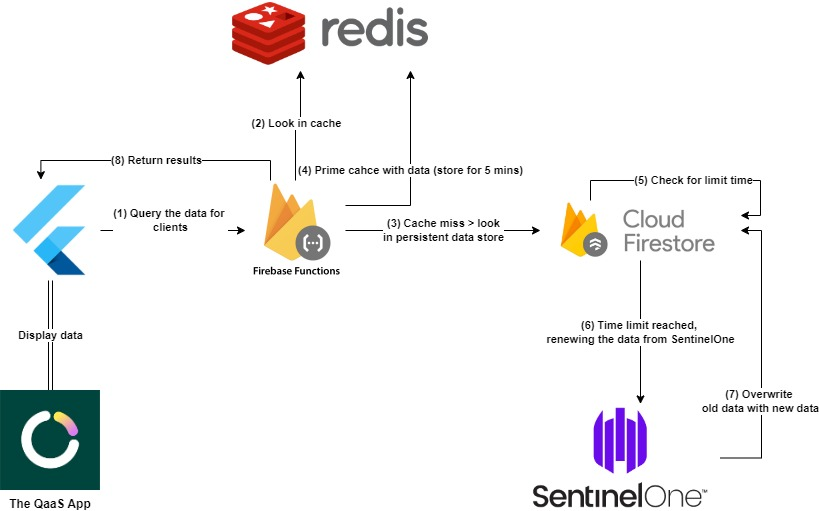
\includegraphics[width=0.9\textwidth]{Figures/Redis Caching.jpg}
  \caption{How the infrastructure would look if Redis is implemented}
\end{figure}


\subsection{Compacting everything into one function}

In the initial phase of the development, the author thought that it was a good idea to make just one function for fetching all data
related to SentinelOne, for the purpose of simplicity for other developers, as there are already more than 50 functions that the
\acrshort{qaas} app has. However, near the end of the development, the author realize that this may not be the best approach because
of the number of requests that one user can make when navigating in the SentinelOne page of the \acrshort{qaas} app. In essence,
when landing through the dashboard, 4 requests already need to be made to fetch the necessary data to be displayed. And every time
the user refreshes that page or navigate back by using the header button in which the traversal process is done by pushing another
route to the navigation stack, therefore calling the \texttt{FutureBuilder} of that page again and making the same 4 initial requests.
After much research, the author found out that Cloud Function v2.0 has no limit on the number of requests that can be made,
(\textit{\cite{firebaseCloudFunctionLimit}}). As for the costing, the price can be increased after the limit of 2 million requests
per month has been exceeded by \$0.40 per million requests (\textit{\cite{pricing}}).

It seems that the issue is not going to make any significant damage to the app, if none. However, if the author needs to be
critical and if given the chance to start over again, the author would have gone to a slightly different approach by separating
the cloud functions into few parts to reduce the number of responsibility that a function must do. This way, the author can
optimize the performance of the app, and make the code more readable and maintainable.
% Modules issue

% N-Central API issue: Not all data is correct
\begin{figure}[htbp]
  \centering
  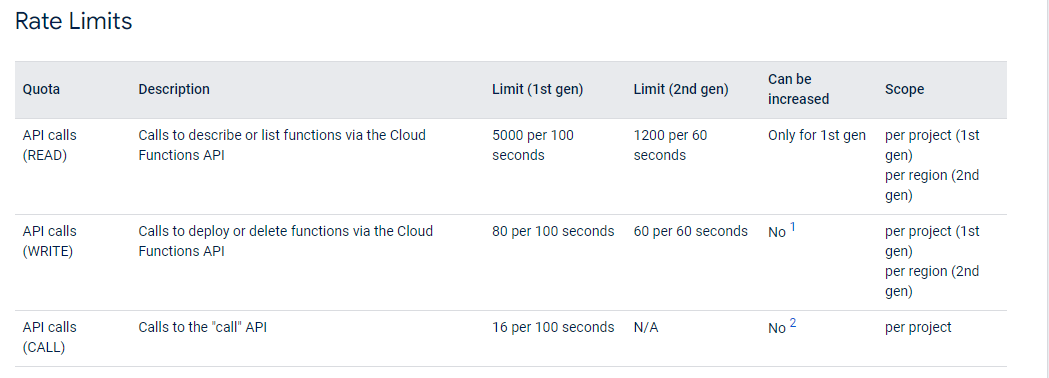
\includegraphics[width=0.9\textwidth]{Figures/Cloud Function no limit.png}
  \caption{The table comparison from the article (\textit{\cite{firebaseCloudFunctionLimit}}) showing that Cloud Function v2.0 has no
    limit on the number of requests that can be made.}
\end{figure}

\begin{figure}[htbp]
  \centering
  
\includegraphics[width=0.9\textwidth]{Figures/Pricing.png}
  \caption{The pricing information for Cloud Function v2.0 (\textit{\cite{pricing}}).}
\end{figure}


% \subsection{Structure of the front-end codebase}

% There are some issues that the author has noticed with the way the \acrshort{qaas} app code was structured. For example, when
% assigning modules to a user, sometimes the user can see the modules that are not assigned to them. This may due to the fact that the
% code is not structured properly, and that they were some bugs left unchecked during the first development of the \acrshort{qaas} app.
% According to the Company Supervisor, the \acrshort{qaas} app itself is still young, so there are many rooms for improvement, especially
% regarding the structure of the codebase and the lack of utilization of software design patterns. The author that there should be a
% separate project, intended directly on refactoring the \acrshort{qaas} app, to make it more robust and scalable in the future.

% Furthermore, there are some inconsistencies in the naming of the variables, especially regarding user tags and user roles. They are
% all doing the same thing, but the naming is different. This due the fact that this project was initially a continuation from an
% unfinished project, and the current developer did not bother to change the naming of the variables. This inconsistency can lead to
% confusion for the future developers, and it is recommended to change the naming of the variables to be more consistent.

% \subsection{Translation}

% The target audience of this project is \acrshort{qict}'s customers, in which all of them are a Dutch company. Therefore, the author and
% the Company Supervisor have tried to make the SentinelOne page in the \acrshort{qaas} to be in Dutch with the text buttons and the
% table headers, and the general \acrshort{ui} widgets. However, as SentinelOne itself is an American company, the data that is fetched
% from the \acrshort{api} is in English. The author and the Company Supervisor have not yet explored the idea of using an external
% package in the back-end that can connect to a translation party, like Google Translate or Microsoft Translator \acrshort{api}, to
% translate the data. This feature, as the stakeholders have mentioned, would be a nice addition to have, as most of the
% clients do not know any technical knowledge of Cybersecurity, and having the data in their native language would make it easier for
% them to better understand the data.

% \subsection{Generate PDF from the data}

% Based on the opinion of a Stakeholder, some pages contain a very important data to the client that they need to be able to download
% the data in a \acrshort{pdf} or Excel format. The author has not yet explored the idea of generating a \acrshort{pdf} from the data
% automatically due to the time constraint.

\subsection{SentinelOne Aggressive Mode}
SentinelOne has a lot of features that can be beneficial for an organization, such as its ability to detect and respond to threats in real-time.
This, however, does not come without its own potential downsides. SentinelOne Agents often exhibit aggressive behaviour, flagging benign and legitimate
files or processes as threats and take actions such as quarantining or mitigating them. This makes them susceptible to false positives,
especially in their default configuration. This can lead to unnecessary disruptions, loss of productivity, and distrust in the security protocol. Organizations
may need to invest some time and resources in investigating and resolving false positives alerts. The author therefore would suggest \acrshort{qict} to
treat it very carefully and to make sure that the SentinelOne Agents are configured properly to avoid unnecessary disruptions.

% \subsection{Future modelling}

% The modelling in both the back-end and front-end are done in a way that is suitable for \acrshort{json} response from the \acrshort{api}.
% However, the author has not yet explored the idea of making the modelling to be more future-proof, by making the modelling to be more
% dynamic, by adding other schemas such as \acrshort{xml}, \acrshort{yaml}, or \acrshort{csv}. This way, the \acrshort{qaas} app can be
% more flexible in the future, and in case SentinelOne wants to also expand their \acrshort{api} server, for example by adding a
% \acrshort{soap} server that returns \acrshort{xml} response.

% \subsection{Compliance with ESLint}

% \subsection{Site Connection Concern}

% During the development of this project, the "Klanten Koppeling" page was used as a medium to connect SentinelOne

